\chapter{Applications} \label{chap:apps}

A couple of applications for the object flow are presented. Firstly, 
in complex video editing and augmented reality, and secondly as part 
of the object-based structure-from-motion. Only visual results are provided 
in both cases.

\section{Video editing}

The video editing that is approached here is the insertion or modification of 
an element in a sequence. For instance, during post-production it is possible that 
an element of a sequence presents inadequate content for the expected audience, and usually 
removing these elements require a hard manual art-edition work. The object flow 
can be exploited in order to reduce drastically the amount of manual work that has to be done. 

The proposed approach is to edit manually the initial frame. The elements of this editing 
can be propagated  through a number of subsequent frames with the object flow. Moreover, 
for complex scenes, with heavy occlusions and sudden illumination changes, several instances 
of the object flow can be used, to take into account the difficult cases. Thus, the overall editing 
work is greatly reduced. Some examples in augmented reality / video editing can be observed in 
Figs. \ref{pt_seg} and \ref{pt_seg2}.

   \begin{figure}[tpbh]
      \centering
      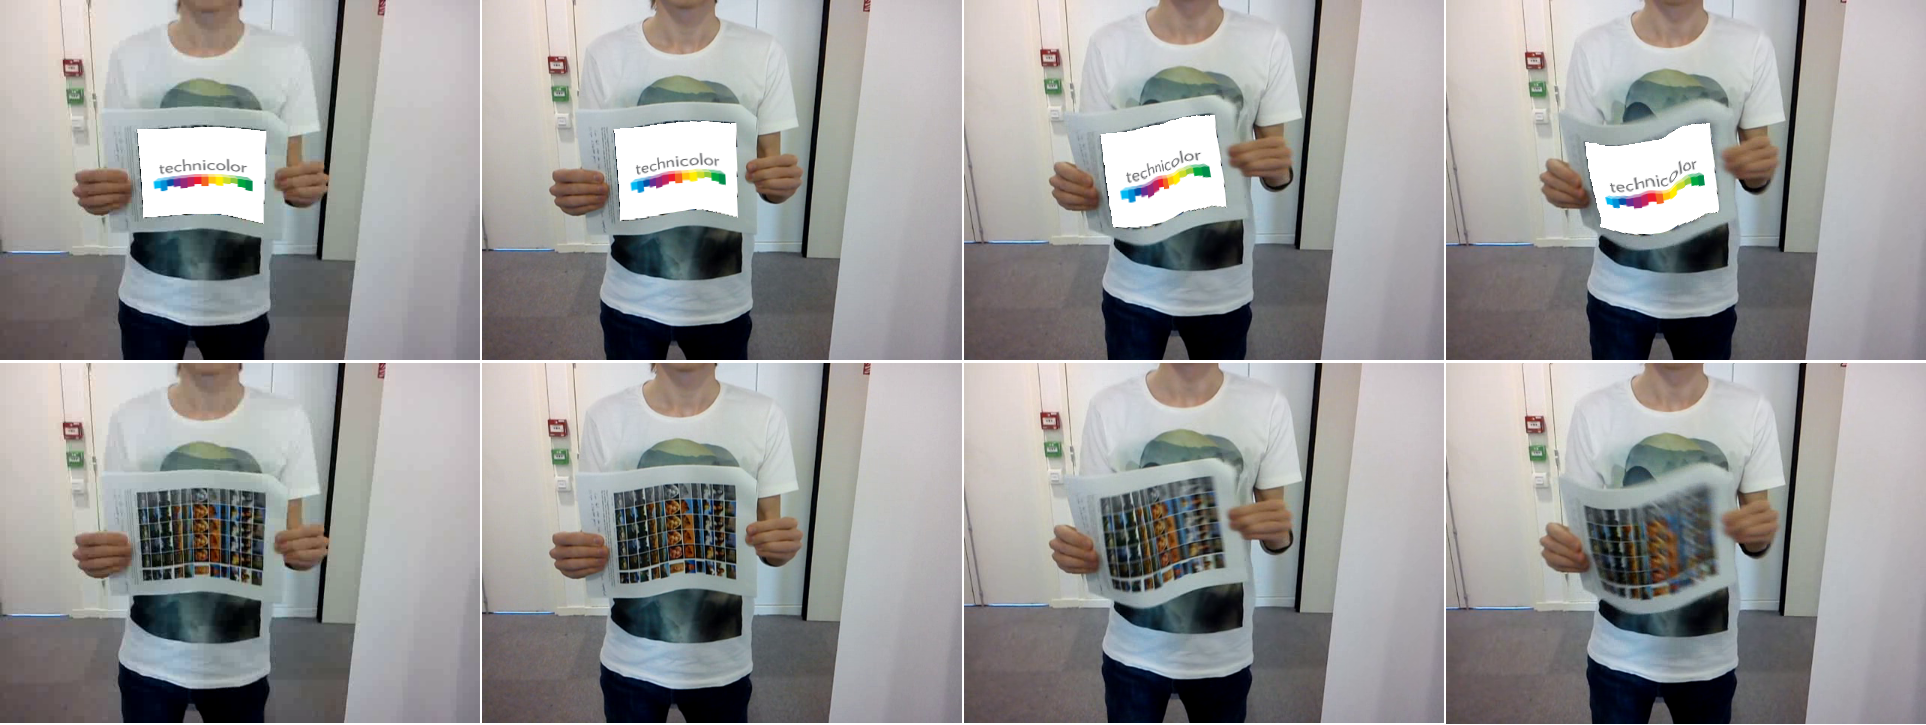
\includegraphics[width=0.95\textwidth]{../images/videoedition.png}
      \caption{  Selected frames in the Dmitry test sequence for video editing. Top: Inserted logo. Bottom: original frames}
      \label{pt_seg}
   \end{figure}

   \begin{figure}[tpbh]
      \centering
      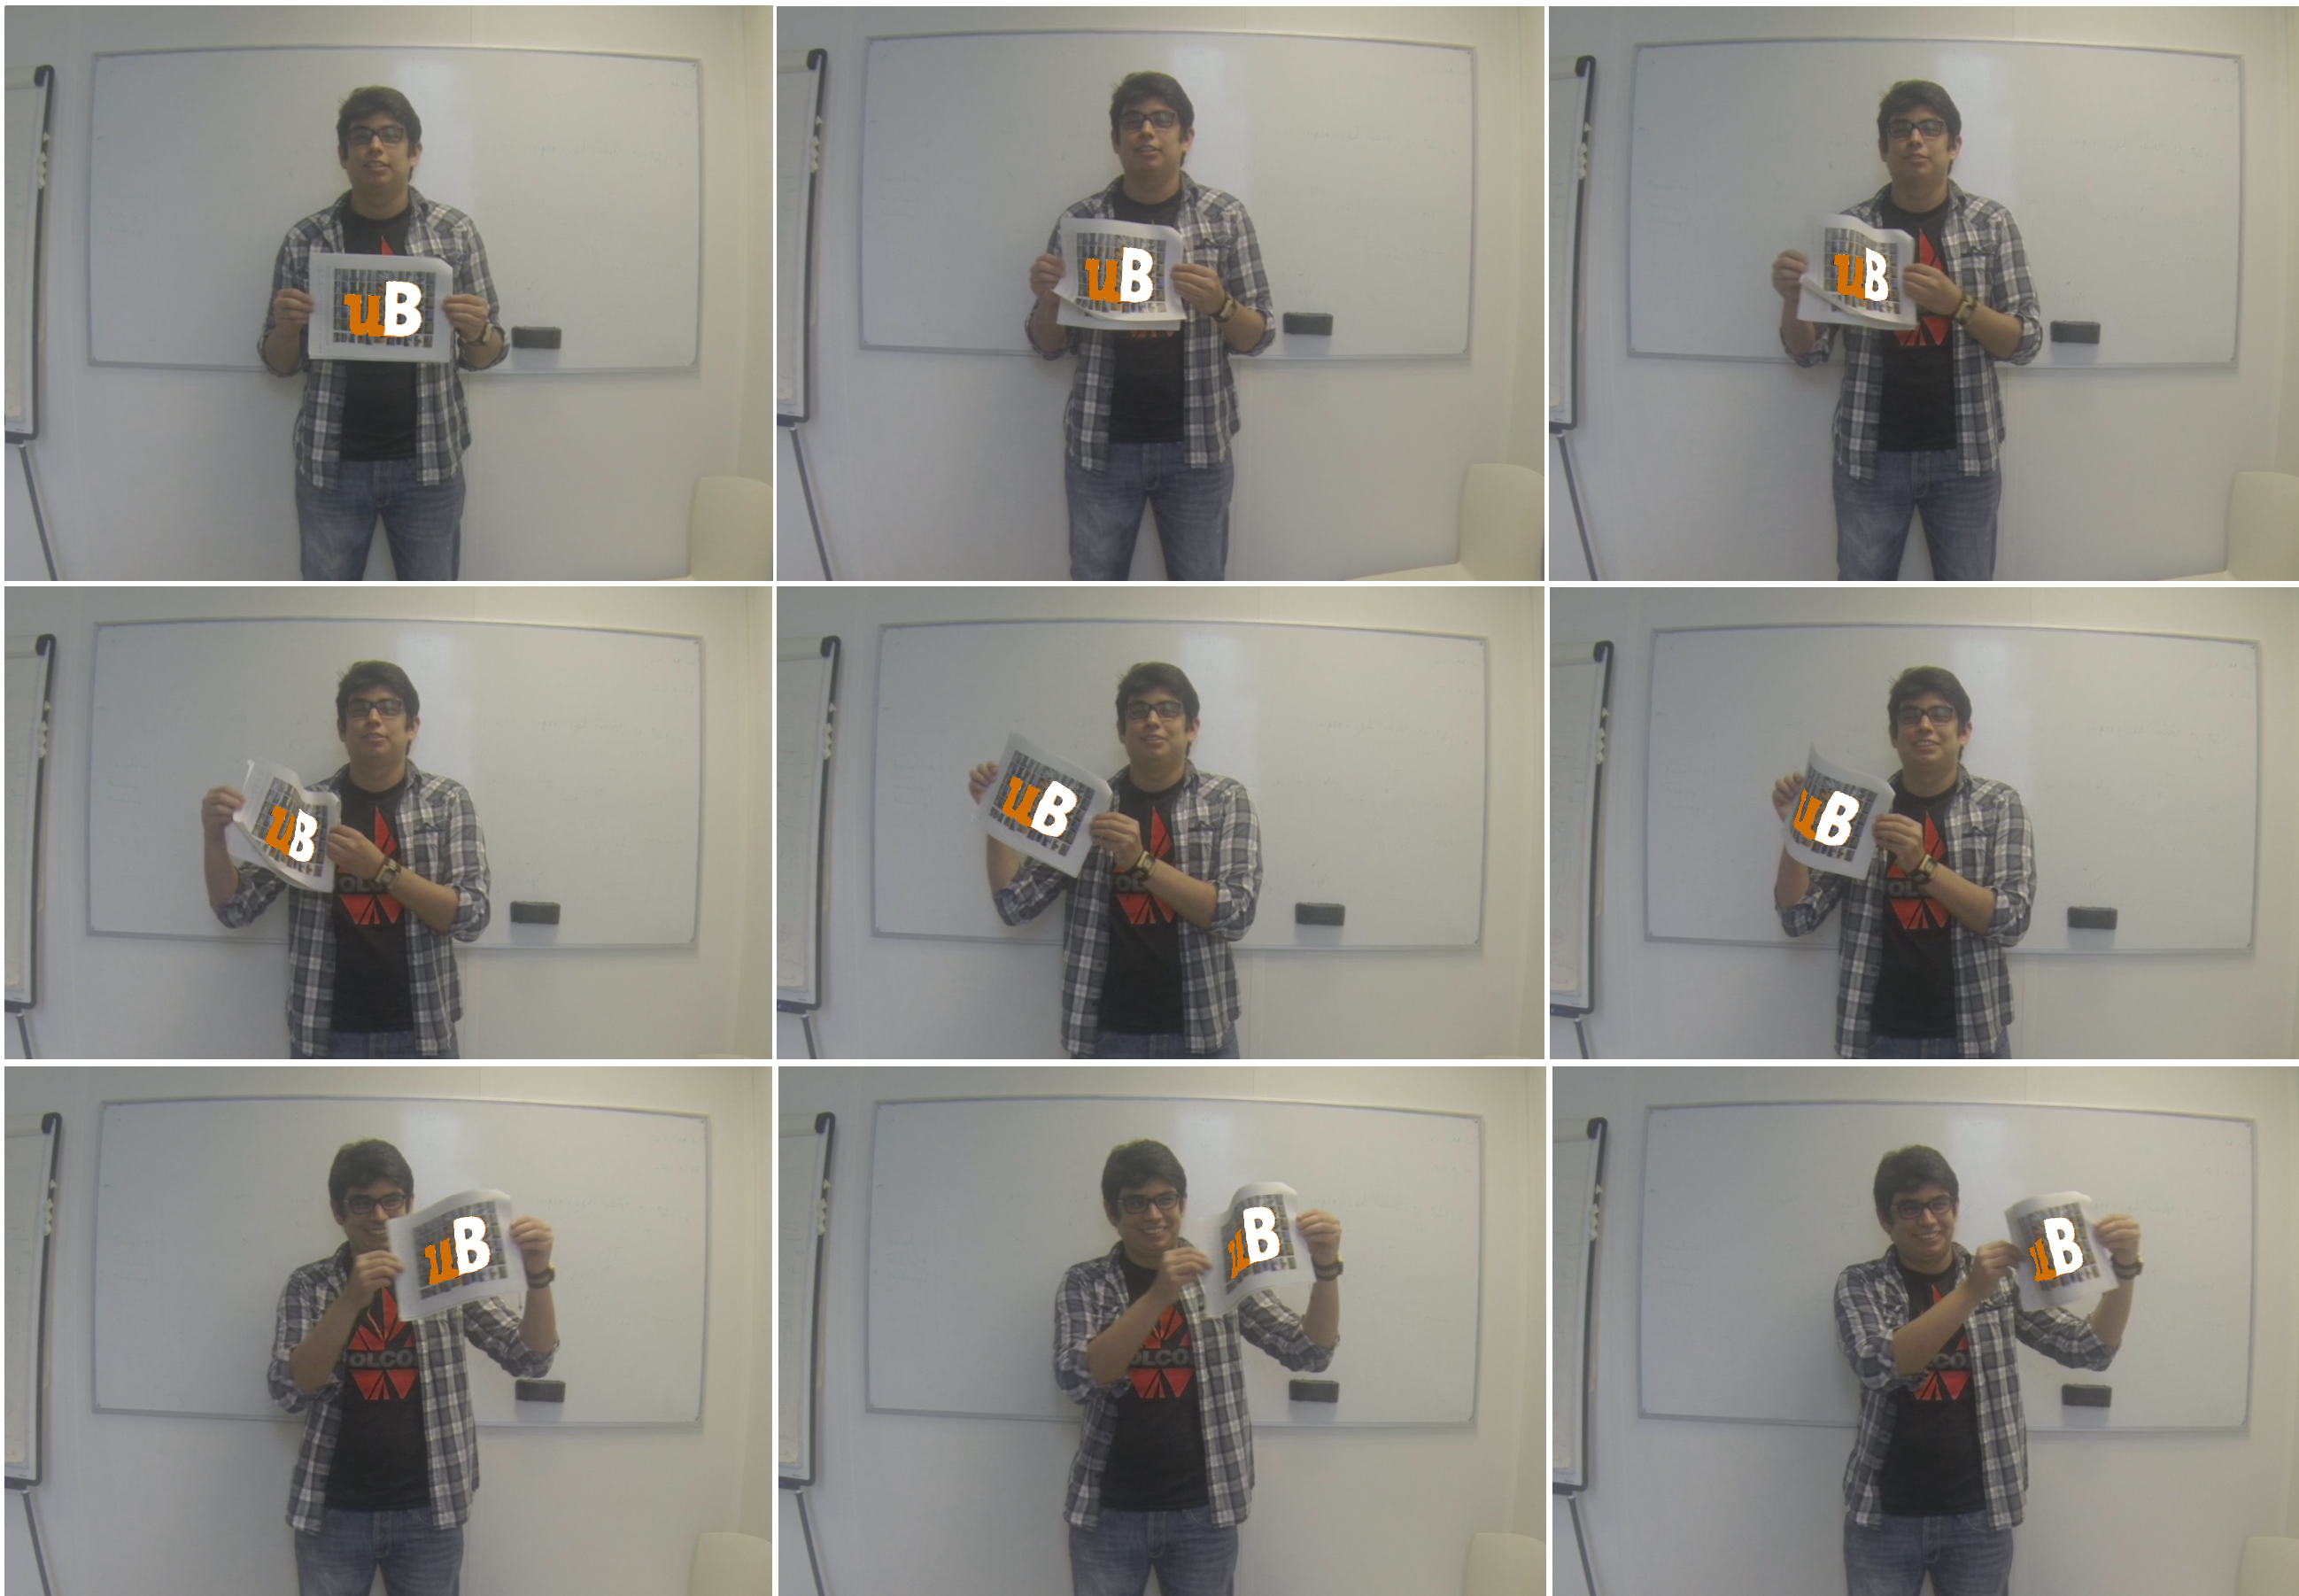
\includegraphics[width=0.95\textwidth]{../images/longUB.png}
      \caption{  Selected frames in the Juan test sequence for video editing. The logo of the University of Burgundy is inserted in the sequence. }
      \label{pt_seg2}
   \end{figure}

\section{Structure from motion}

The idea of the structure from motion problem ({\it SfM}) is to 
recover the shape of objects or scenes from a sequence of images obtained from a camera that follows certain motion. Usually, it is assumed that 
the scene contains rigid objects undergoing an 
Euclidean motion \cite{c43}.

The most common way to solve the {\it SfM} is to 
find a set of correspondences between the acquired 
frames by using a feature matching method, and use the epipolar geometry constraint for two images 
($x_1^T E x_2 = 0$). Usually, the {\it 8 points algorithm} is used to obtain a relative rotation 
and translation of the camera by factorizing the 
essential matrix ($E$). However, given the simplicity of the approach, the algorithm is very sensitive to noise and several other approaches have 
been proposed: {\it 7 points} or {\it 5 points} algorithms are at hand. Nevertheless, one of the major weakness of such 
methods is still the feature matching (w.r.t precision and sparsity) \cite{c43}. 

When matching is replaced by optical flow, the 
scene structure and the camera motion are tied 
together by the equation:

\begin{equation}
\textbf{u}(x) = A(x)\textbf{v}/Z + B(x)\omega ,
\label{eq_dfc}
\end{equation}
%\begin{center}
 where, $ A =  \left[ {\begin{array}{ccc} 1 & 0 & -x\\ 0 & 1 & -y \end{array} } \right]$, 
 and, $ B =  \left[ {\begin{array}{ccc} -xy & (1+x^2) & -y\\ -(1+y^2) & xy & x \end{array} } \right]$.
%\end{center}

In Eq. \ref{eq_dfc}, $\omega$ is 
the camera angular velocity, and $\textbf{v}$ is the camera linear velocity. 
The 3D point position is 
 $\textbf{X}=[X,Y,Z]$, and its 
 projection over the focal plane is 
 $\textbf{x}=[x,y]$.
 

The optical flow, however, has been traditionally 
inaccurate for long term point tracking, and due to the fact that an optimal structure in the least square sense can 
be obtained from camera velocities (which are more accurately extracted from the flow), the research was 
mainly focused on capturing camera ego-motion \cite{c43}. 

   \begin{figure}[tpbh]
      \centering
      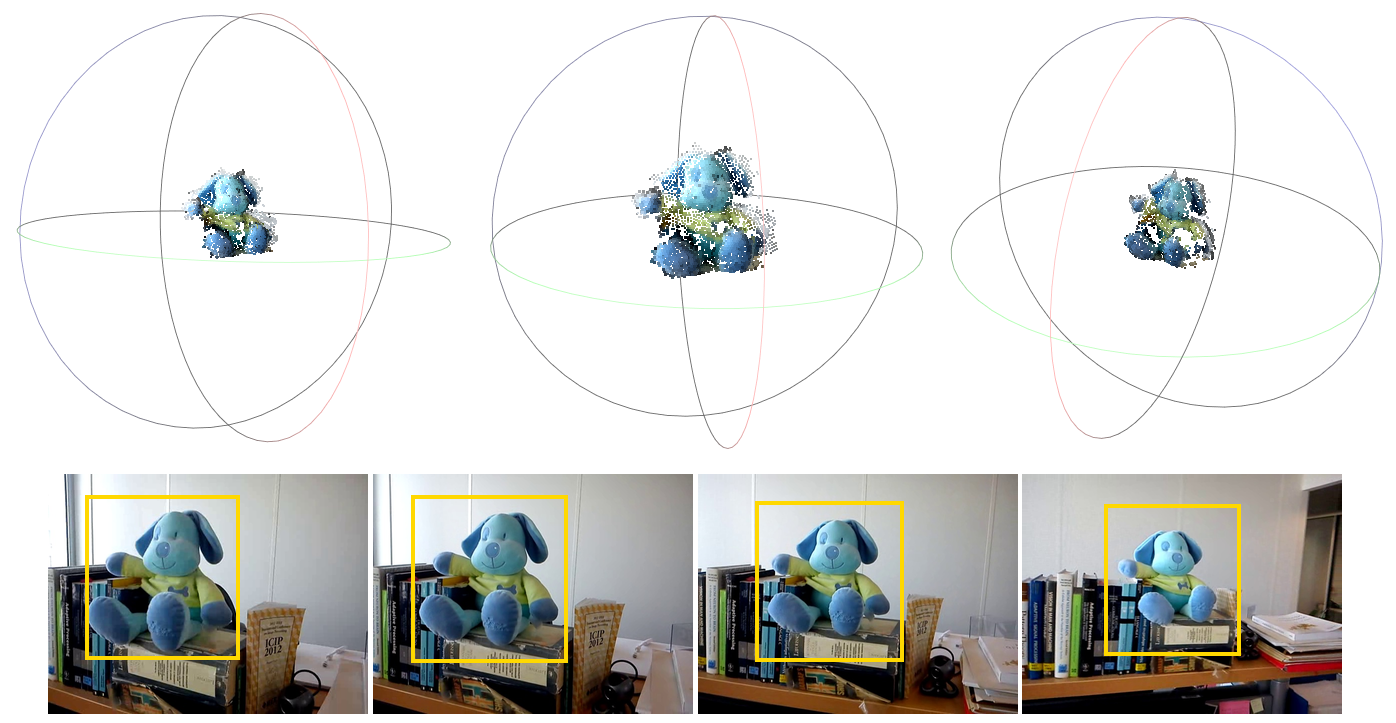
\includegraphics[width=0.95\textwidth]{../images/SFM2.png}
      \caption{ SFM based on the object flow matches in the Puppy dataset. Top: views of the computed structure. Bottom: Used frames. }
      \label{sfm2}
   \end{figure}
   
As it has been demonstrated that the object flow 
increases accuracy of the point trajectories estimation, it can be connected to a {\it SfM} 
pipeline as point matching method, not only as camera motion direct estimator. Some results can be appreciated in Figs. \ref{sfm2} and \ref{sfm3}. These results are generated 
by using the Changchang Wu's public tools based on his work on Linear-Time Incremental Structure From Motion \cite{c42} and sets of matches generated 
with the object flow between pairs of frames. Fig. \ref{sfm4} shows the results of the reconstruction by extracting sift features between frames (not only consecutive pairs). It can be 
appreciated, by analyzing  Fig. \ref{sfm3} and Fig. \ref{sfm4}, that the object flow matches, being of dense nature, can be used to obtain a more dense structure of the interest object. 
On the other hand, the Sift matches between pairs of frames provide a less dense reconstruction if only the interest object is taken into account. However, the Sift matches offer a global 
structure, by not taking into account only matches inside the interest region, and some elements of the environment are also reconstructed, including a  better reconstruction of the shoulders. 
It is worth pointing out, then, that both kind of matches offer advantages, and the feature election becomes a matter of the specific needs of the application. 
   
   \begin{figure}[tpbh]
      \centering
      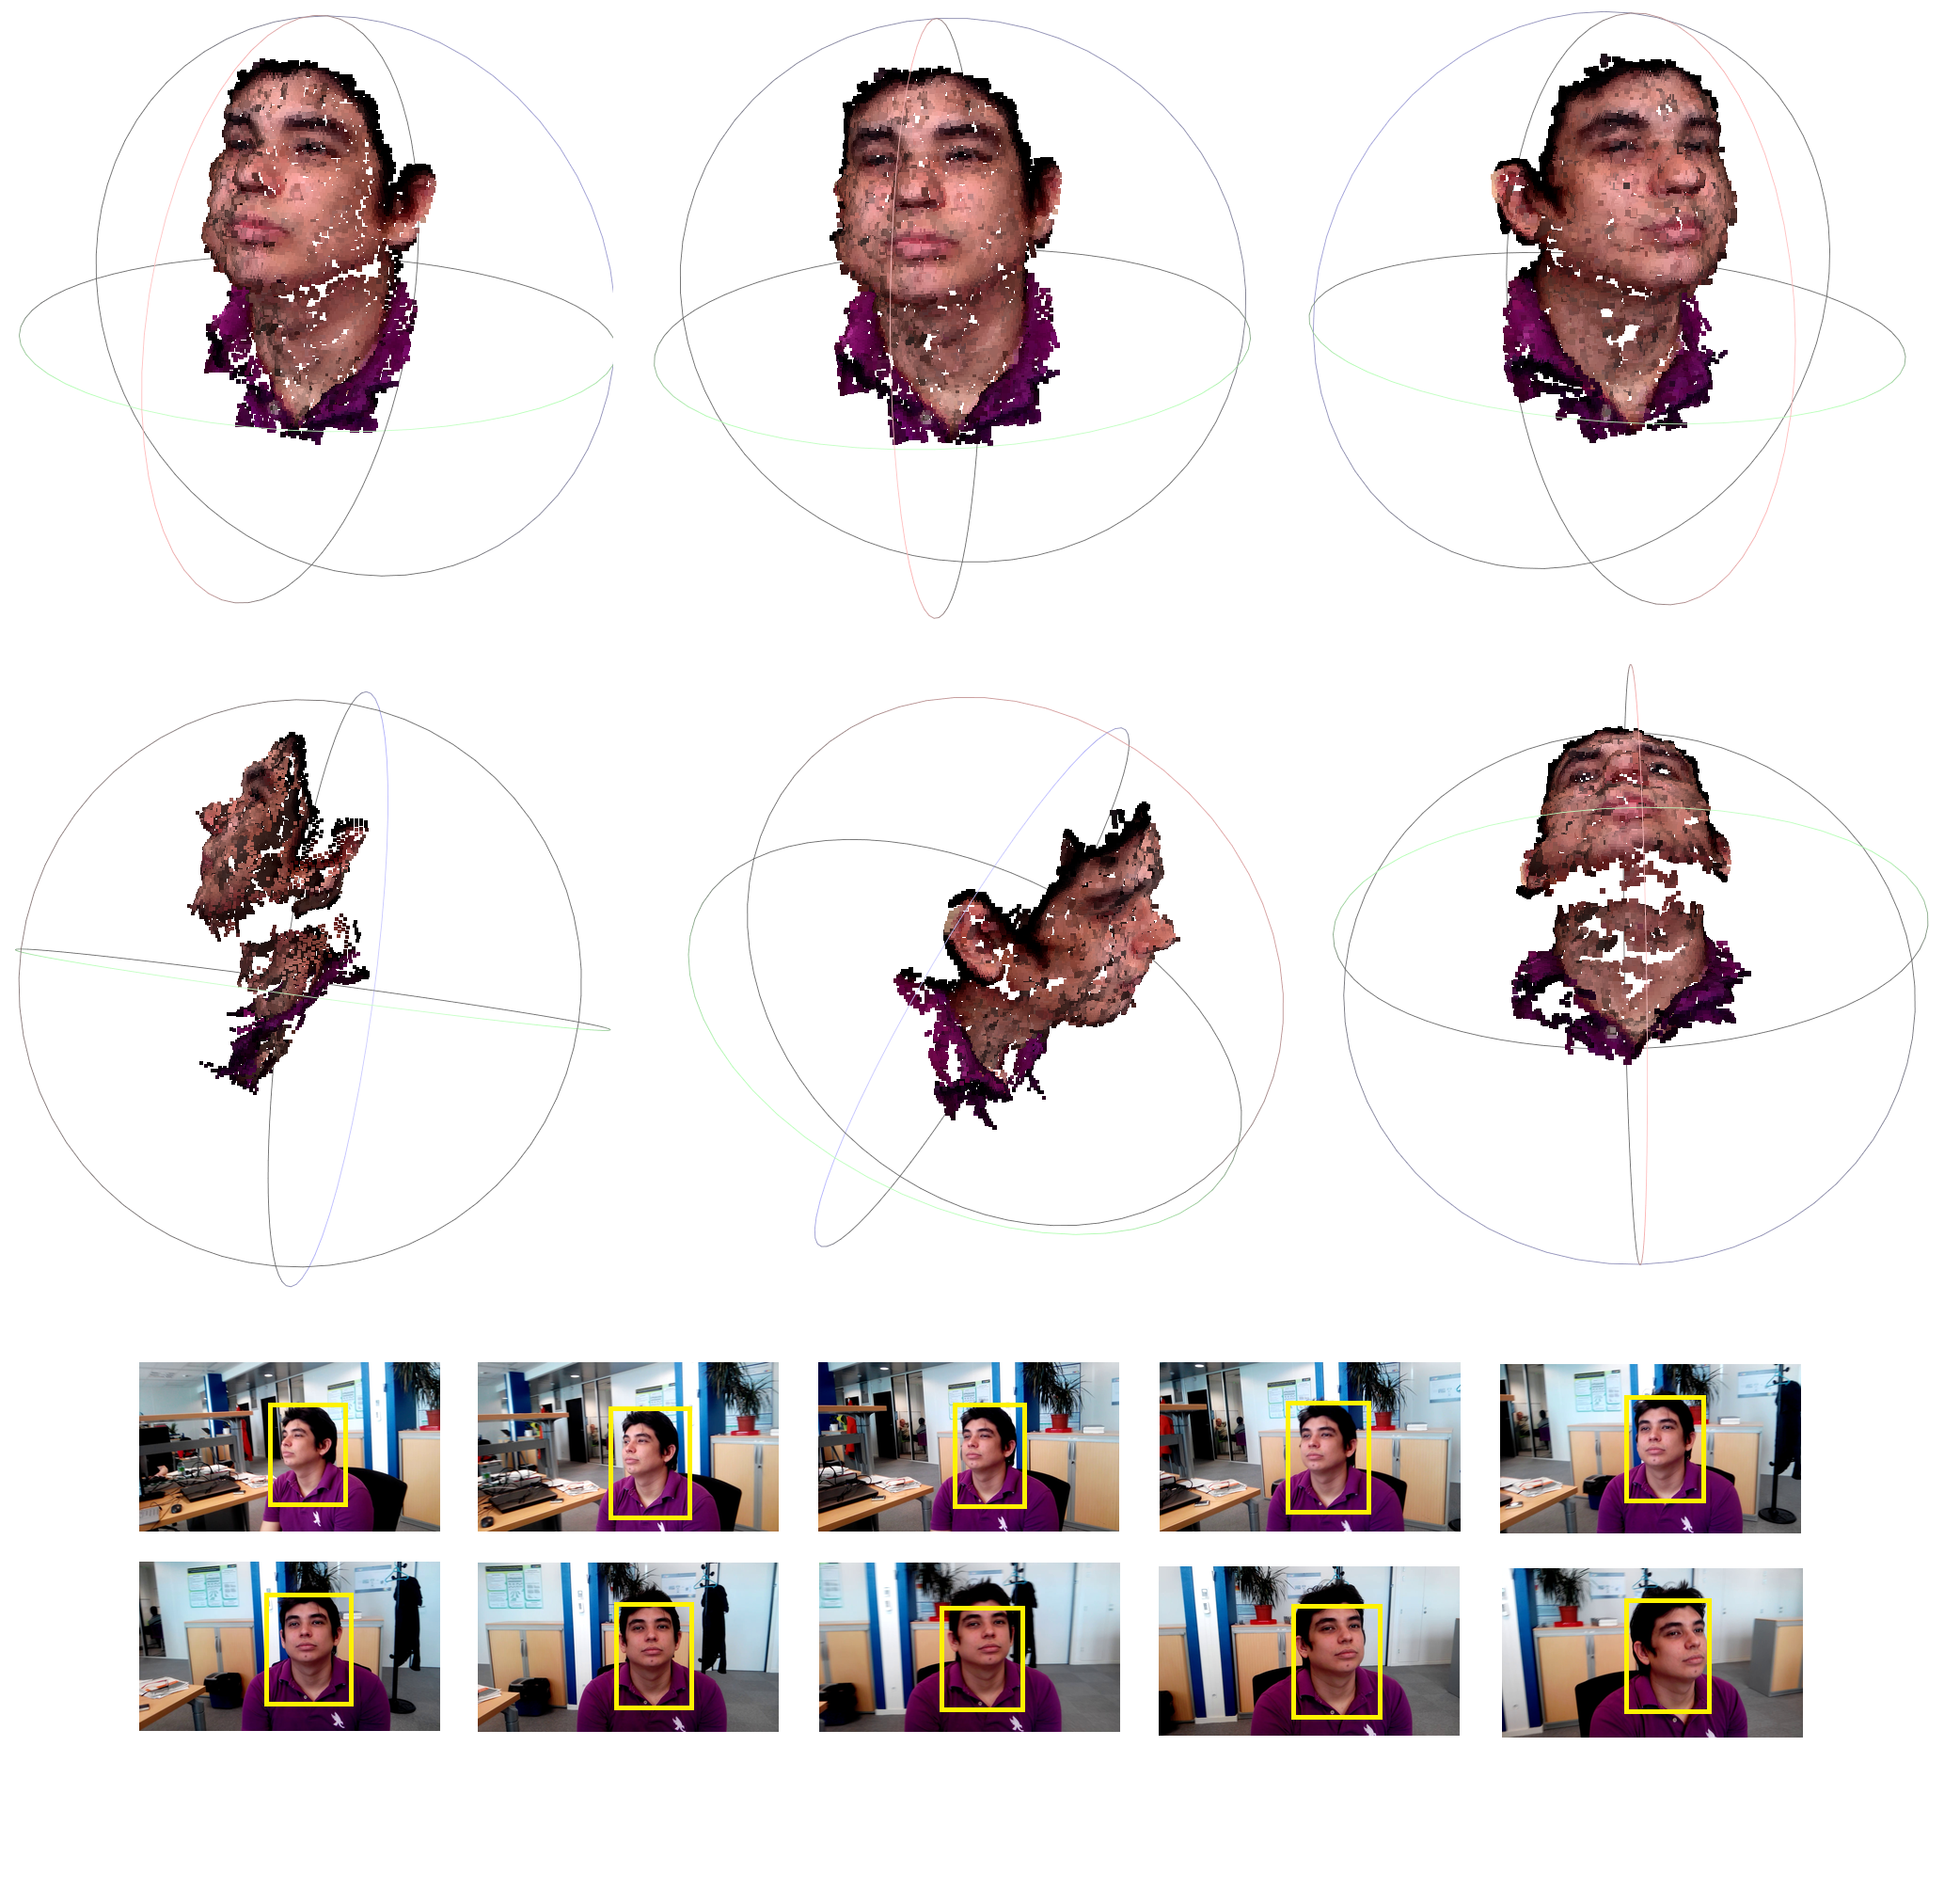
\includegraphics[width=0.95\textwidth]{../images/SFM3_1.png}
      \caption{ SFM based on the object flow matches in the JuanFace dataset. Top: views of the computed structure. Bottom: Used frames. }
      \label{sfm3}
   \end{figure}

   \begin{figure}[tpbh]
      \centering
      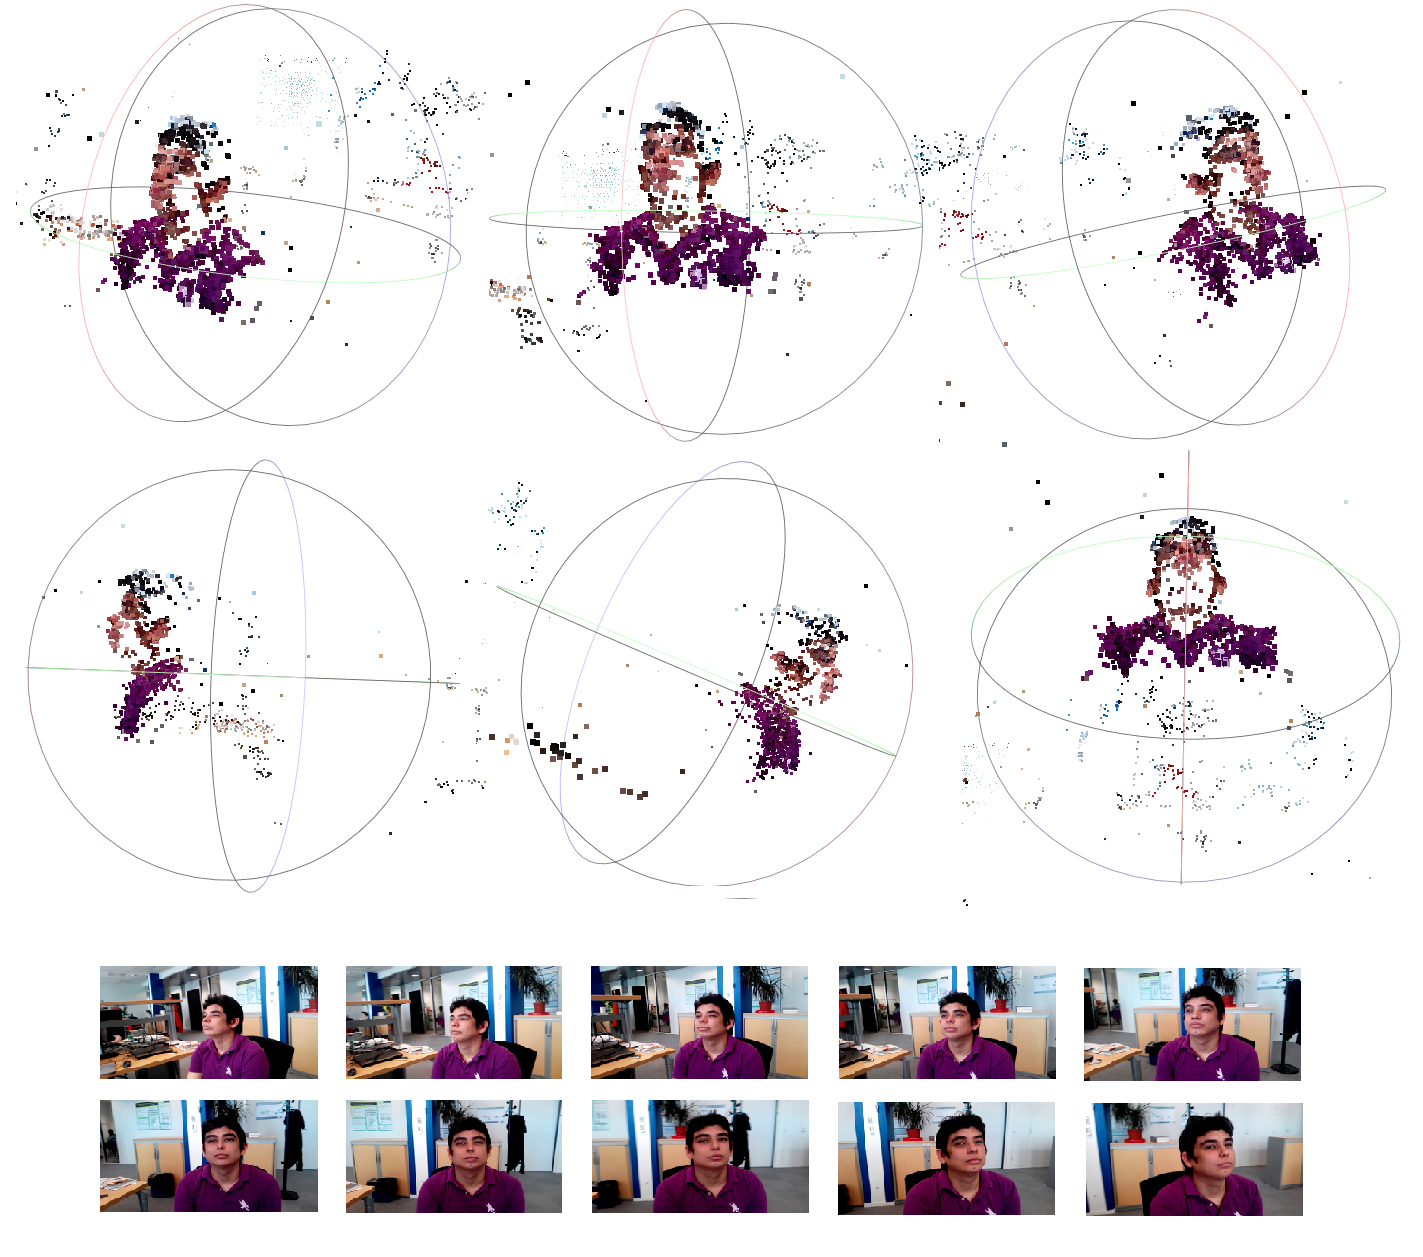
\includegraphics[width=0.95\textwidth]{../images/SFM3_2.png}
      \caption{ SFM based on the Sift matches between frames. Top: views of the computed structure. Bottom: Used frames. }
      \label{sfm4}
   \end{figure}
